%!TEX TS-program = xelatex
\documentclass{nirev-cv}
\addbibresource{bibliography.bib}

\usepackage{ulem}


\begin{document}
\header{Guilherme}{DeMaio}
       {Software Developer}

%\usetikzlibrary{calc}
%\begin{tikzpicture}[remember picture,overlay]
%  \node[anchor=north west,inner sep=0pt] at ($(current page.north west)-(2cm,5cm)$) {
%     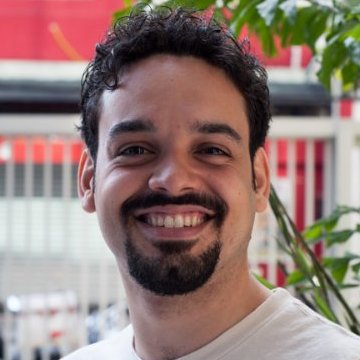
\includegraphics[width=4cm]{profile.jpg}
%  };
%\end{tikzpicture}

% In the aside, each new line forces a line break
\begin{aside}
  %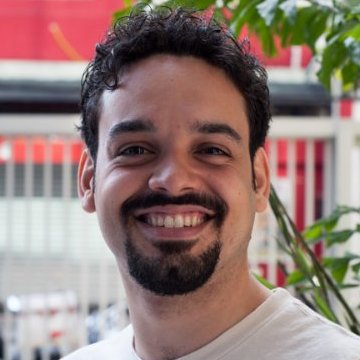
\includegraphics[width=4cm]{profile.jpg}
  \section{contact}
    R. Ministro Gastão Mesquita, 257
    05012-010 São Paulo
    Brasil
    ~
    +55 11 9 8393 2639
    {\faSkype } guilherme\_nirev
    \href{mailto:guilherme@nirev.org}{guilherme@nirev.org}
    \href{http://nirev.org}{http://nirev.org}
    \href{https://github.com/nirev}{\faGithub /nirev}
    \href{https://twitter.com/nirev}{\faTwitter /nirev}
    \href{https://linkedin.com/in/nirev}{\faLinkedin /nirev}
  \section{languages}
    native portuguese
    fluent english
    basic french
  \section{programming}
    Elixir, Java, Ruby, Javascript, C, Python,
    HTML, css, bash,
    Kafka, Spark, docker, 
    monitoring tools
  \section{interests}
distributed systems, making a better world, data structures, music, martial arts, science fiction books
\end{aside}

\section{about me}

I've been developing software for 10 years, from web apps to embedded media applications.
During this time I've come to believe that:
- Empathy first, always
- Trust is key
- Less is more

On the tech side of things, I'm more of a backend/operations type, but I do dabble a bit on the frontend.
I enjoy taking part and ownership of where and how applications are deployed and monitored.

I take pride in being part of team. I enjoy giving talks and getting to know people at conferences.
I've been a team lead before, and I dislike the term "soft skills". Once you're in a position as such, those so called "soft" skills are exactly what is most important. 

\section{recent experience}
\workentry
    {September 2015}{*}
    {Senior Software Engineer at XERPA}
    {São Paulo - Brazil}
    {I joined the company as their first employee to help build the SaaS platform tackling HR bureaucracy in Brazil.
    We started from day-0 with Elixir and Phoenix on the backend, with the frontend initially in simple html/css/jquery. We eventually migrated the frontend to ClojureScript using a GraphQL API.
    
    Among things I took part are: \\ \small
    - Bootstrapped the platform using Elixir, Phoenix and PostgreSQL \\
    - Managing infrastructure with Terraform and Ansible \\
    - Built libraries for: \\
    - Authentication and Authorization \\
    - Indexing things to ElasticSearch, as well as defining mappings \\
    - Resizing and manipulating images \\
    - Integrating with payment gateways \\
    - Defining and prioritizing features together with product and business/sales teams. I also did visit "beta" clients in the beginning to get a better understanding of the problems we needed to solve. \\
    - Collaborating heavily with Customer Success team to help streamline client usage after signup, focusing on quickly solving bugs and creating stories to improve the user experience \\
    - Using OCR to identify unique numbers in PDFs, built a document distribution feature which greatly improved sales and customer satisfaction.} 

\workentry
  {November 2012}{September 2015}
  {Team Lead (Search and Analytics) at Elo7}
  {São Paulo - Brazil}
  {A marketplace with high traffic and transaction volume. The stack was based on Java, Ruby and Scala on AWS infrastructure. A fast paced environment, with agile practices, and focusing on delivering fast with quality. We measured and logged using StatsD, Graphite, and NewRelic, and deployed constantly. I was leading the Search and Analytics Team: a small team using Solr, Kafka and Spark to improve search and real time reports, and responsible for its infrastructure and pipeline tools.}


\subsection{past experiences}
details available upon request

\begin{entrylist}

\shortworkentry
  {04/2012}{10/2012}
  {Intern at INRIA Paris-Roquencourt}
  {Paris - France}
  {Research on fault-tolerance requirements for Wireless Sensor Networks macroprogramming.}

\shortworkentry
  {03/2011}{09/2012}
  {Undergrad Researcher at USP - CHOReOS project}
  {São Paulo - Brazil}
  {Research and implementation involving: choreography analysis using graph metrics,
  dynamic adaptation techniques, implementation of a testing framework, and cloud computing.}

\shortworkentry
  {08/2010}{02/2011}
  {Software Developer (C/C++) at RR Sistema}
  {Vitória/ES - Brazil}
  {Porting their implementation of Brazilian DTV middleware to different platforms.
  Mainly programming in C/C++, with low-level and multimedia libraries (GStreamer, DirectFB, pthreads, osal, etc),
  and required knowledge of the Brazilian digital television standards.}

\shortworkentry
  {01/2009}{12/2010}
  {Undergrad Intern at Multimedia and Network Research Lab}
  {Vitória/ES - Brazil}
  {Working with the Brazilian DTV middleware; ported it for Android. }

\shortworkentry
  {08/2008}{12/2008}
  {Undergrad Intern at LASSY}
  {University of Luxembourg - LU}
  {RESIST project: developed a prototype for SOA eHealth application with multiple services.}

% \shortworkentry
%   {January 2008}{March 2008}
%   {Intern at CISA Trading S.A.}
%   {Trading company, São Paulo/SP - Brazil}
%   {Maintaining their internal software solution which manages all of the companies processes.
%   The system was written in the Progress4GL language.}

\shortworkentry
  {03/2007}{12/2007}
  {Undergrad Intern at NINFA laboratory}
  {Vitória/ES - Brazil}
  {Joint project with ESCELSA, state's electric power utility, building automated classifiers
  for finding frauds done by its clients. Used optimization heuristics, neural networks and clustering.
  Tools developed in Java, C++ and Matlab.}

\shortworkentry
  {09/2006}{03/2007}
  {PHP Developer at Lettera Soluções}
  {Vitória/ES - Brazil}
  {Developing and managing web sites using CSS, (x)HTML, PHP, ASP, MySQL, PostgreSQL, as well as common Linux admin tools.}
\end{entrylist}


\section{education}
 
\begin{entrylist}
  \entry
    {2011–2014}
    {Master in Computer Science}
    {University of São Paulo - Brazil}{}
  \entry
    {2005–2010}
    {B.Sc. in Computer Science}
    {Federal University of Espírito Santo - Brazil}{}
\end{entrylist}

\printbibsection{article}{article in peer-reviewed journal}
\printbibsectionpar{inproceedings}{international peer-reviewed conferences/proceedings}{notkeyword={brazil}}
\printbibsectionpar{inproceedings}{local peer-reviewed conferences/proceedings}{keyword={brazil}}
\printbibsection{misc}{other publications}
\printbibsection{report}{research reports}

\end{document}
